\begin{itemize}
 \item The naive Bayes approach makes the simple assumption that all the attributes are independent. This leads to a much simpler, though surprisingly effective classifier in practice.
 \item The naive Bayes classifier uses the sample mean and a diagonal sample covariance matrix for each class $c_i$ . Thus, in total 2d parameters have to be estimated, corresponding to the sample mean and sample variance for each dimension $X_j$ .
\begin{figure}[H]
\centerline{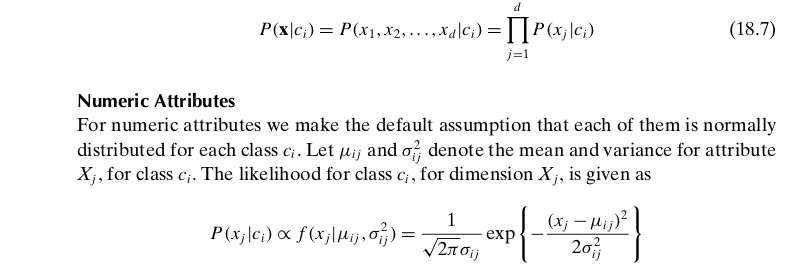
\includegraphics[width=1.2\textwidth]{Figures/naive}}
\caption{\label{fig:figure21}Likelihood Estimation in Naive Bayes ,Numeric}
\end{figure}
\begin{figure}[H]
\centerline{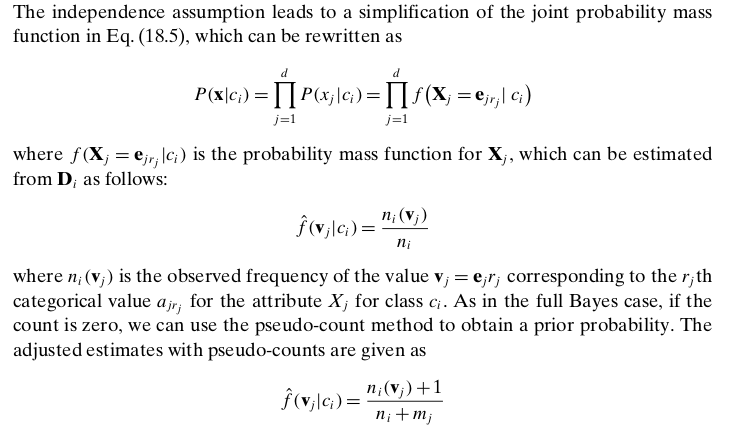
\includegraphics[width=1.1\textwidth]{Figures/naive2}}
\caption{\label{fig:figure22}Likelihood Estimation in Naive Bayes ,Categorical}
\end{figure}
\begin{figure}[H]
\centerline{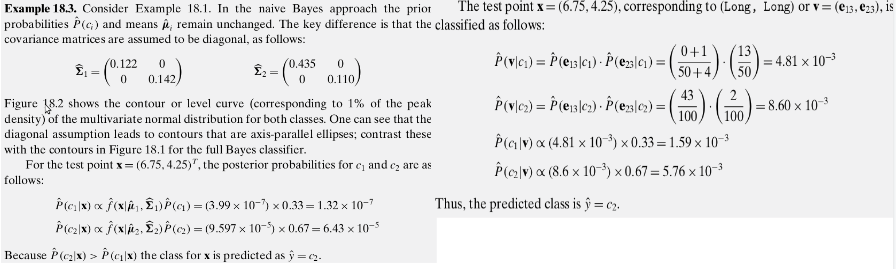
\includegraphics[width=1.7\textwidth]{Figures/bayes4}}
\end{figure}
\end{itemize}